\chapter{Herramientas}\label{ch:herramientas}

En este capítulo se abordarán las diferentes herramientas,
tanto generales como específicas para el entorno \textit{MIPS32},
presentes en \textit{JAMS}.


\section{Explorador}\label{sec:explorador}

El explorador es la \textbf{herramienta más importante de todo el editor}.
Permite \textbf{visualizar las carpetas y archivos del proyecto}
de una manera rápida y sencilla.
El explorador es una herramienta pensada para que cualquier tipo de proyecto
pueda implementar su version de una manera rápida y sencilla.
La tecnología detrás del explorador se \textbf{usa en diferentes partes de la aplicación},
como pueden ser la sección de acciones y las herramientas de etiquetas y archivos
a ensamblar.

\begin{figure}[H]
    \centering
    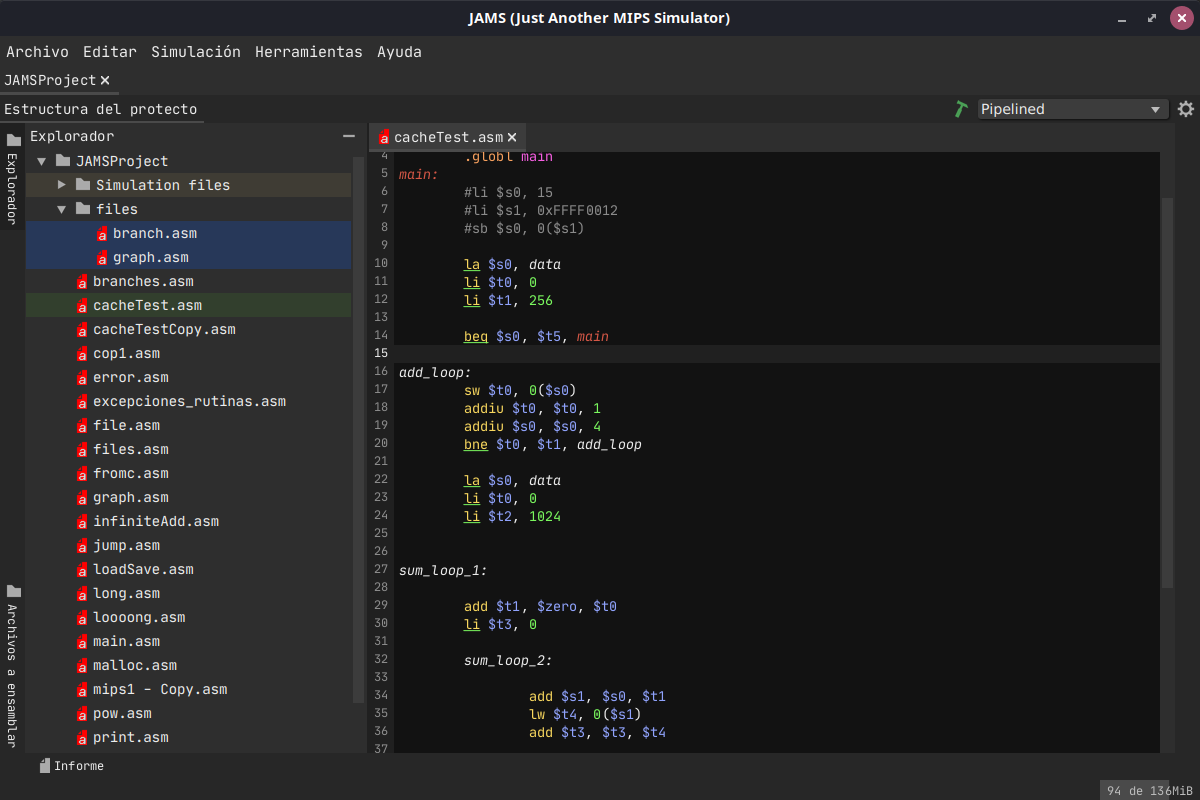
\includegraphics[width=0.8\textwidth]{images/tools/jams-explorer}
    \caption{Explorador}
    \label{fig:jams-explorer}
\end{figure}

\noindent El explorador presenta las siguientes funcionalidades:
\begin{itemize}
    \item \textbf{Abrir archivos:} la principal funcionalidad del editor
    es poder abrir archivos en el editor.
    Haciendo doble clic en un archivo o seleccionándolo y pulsando
    $enter$, se mostrará un editor especializado para el archivo
    en cuestión.
    \item \textbf{Desplazamiento:} el usuario puede desplazarse por el
    explorador utilizando las flechas del teclado.
    El usuario también puede ir seleccionando archivos mientras se
    mueve manteniendo pulsado la tecla $shift$.
    \item \textbf{Selección:} el usuario también puede seleccionar
    elementos del explorador de manera selectiva manteniendo
    pulsada la tecla $ctrl$ mientras se emplea el botón principal
    del ratón en los elementos a seleccionar.
    \item \textbf{Menú de contexto:} el menú de contexto muestra
    una lista de acciones aplicables a la selección.
    El usuario podrá desplegar este menu usando el botón secundario
    del ratón.
\end{itemize}

\noindent El explorador de archivos es un explorador específico
que le permite al usuario visualizar la estructura del proyecto
actual.
Este explorador mostrará sus elementos con un fondo diferente en
casos especiales:
\begin{itemize}
    \item \textbf{Azul:} el elemento está seleccionado.
    \item \textbf{Verde:} el elemento está dentro de la lista de
    archivos a ensamblar.
    \item \textbf{Verde azulado}: el elemento está seleccionado y
    dentro de la lista de archivos a ensamblar.
    \item \textbf{Marrón:} el elemento no es considerado
    parte del proyecto.
\end{itemize}


\section{Archivos a ensamblar:}\label{sec:archivos-a-ensamblar:}

La herramienta de archivos a ensamblar permite
ver, ordenar, eliminar y modificar los \textbf{archivos que se van a ensamblar}.

\begin{figure}[H]
    \centering
    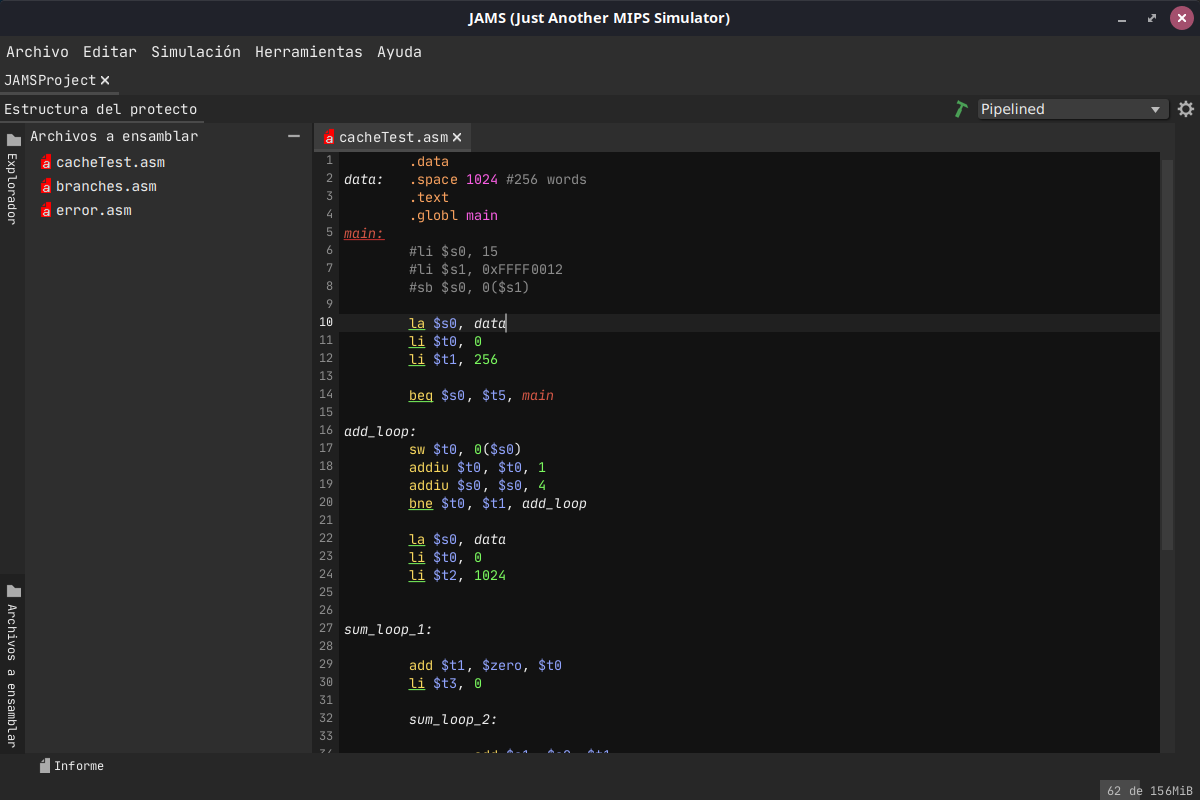
\includegraphics[width=0.8\textwidth]{images/tools/jams-files-to-assemble}
    \caption{Archivos a ensamblar}
    \label{fig:jams-files-to-assemble}
\end{figure}

\noindent Pueden haber tipos de proyecto donde el
orden de los archivos a ensamblar importe.
Esta herramienta permite al usuario \textbf{ordenar los archivos}
a ensamblar \textbf{arrastrándolos a la posición deseada}.
La herramienta también permite \textbf{eliminar un archivo} de la lista
mediante un menú de contexto que el usuario puede abrir usando
el botón secundario del ratón en el archivo a eliminar.


\section{Informe}\label{sec:informe}

La herramienta \textbf{informe} te permite \textbf{visualizar el resultado}
de los ensamblajes que hagas en tu proyecto.
También le permite a otras herramientas informar sobre cambios de estados y errores.

\begin{figure}[H]
    \centering
    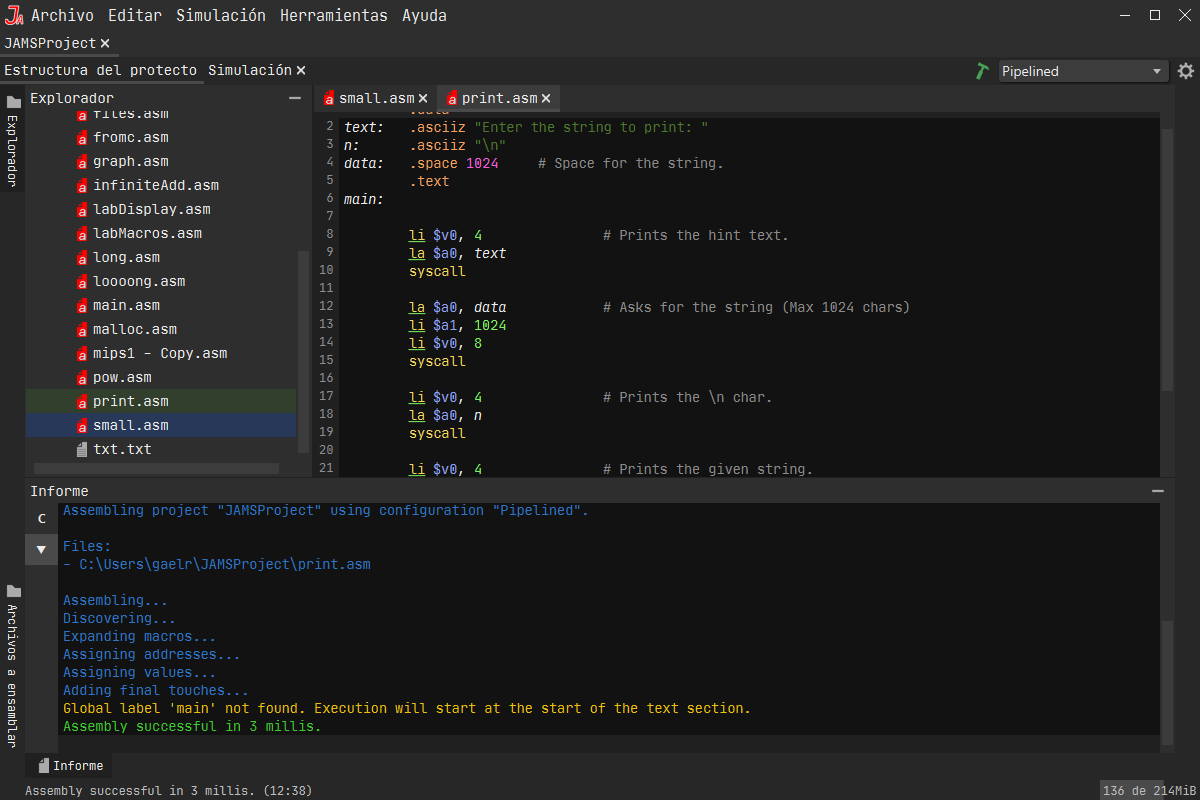
\includegraphics[width=0.8\textwidth]{images/tools/jams-log}
    \caption{Informe}
    \label{fig:jams-log}
\end{figure}

\noindent El informe contiene dos botones con el que se puede interactuar:
\begin{itemize}
    \item El botón $C$ permite limpar el informe, eliminando todo el
    texto presente en él.
    \item El botón $\nabla$ permite habilitar o deshabilitar el desplazamiento
    automático al final del visualizador.
    Si esta opción está habilitada, el visualizador se desplazará
    automáticamente hasta el final del visualizador cuando un
    nuevo mensaje entra en él.
\end{itemize}


\section{Memoria}\label{sec:memoria-herramienta}

La herramienta \textbf{memoria} permite visualizar la información que
contiene la memoria y las cachés de un simulador en el estado actual.
Esta herramienta muestra la memoria en celdas de 4 bytes,
lo cual permite una visualización óptima para arquitecturas
basadas en 32 bits.

\begin{figure}[H]
    \centering
    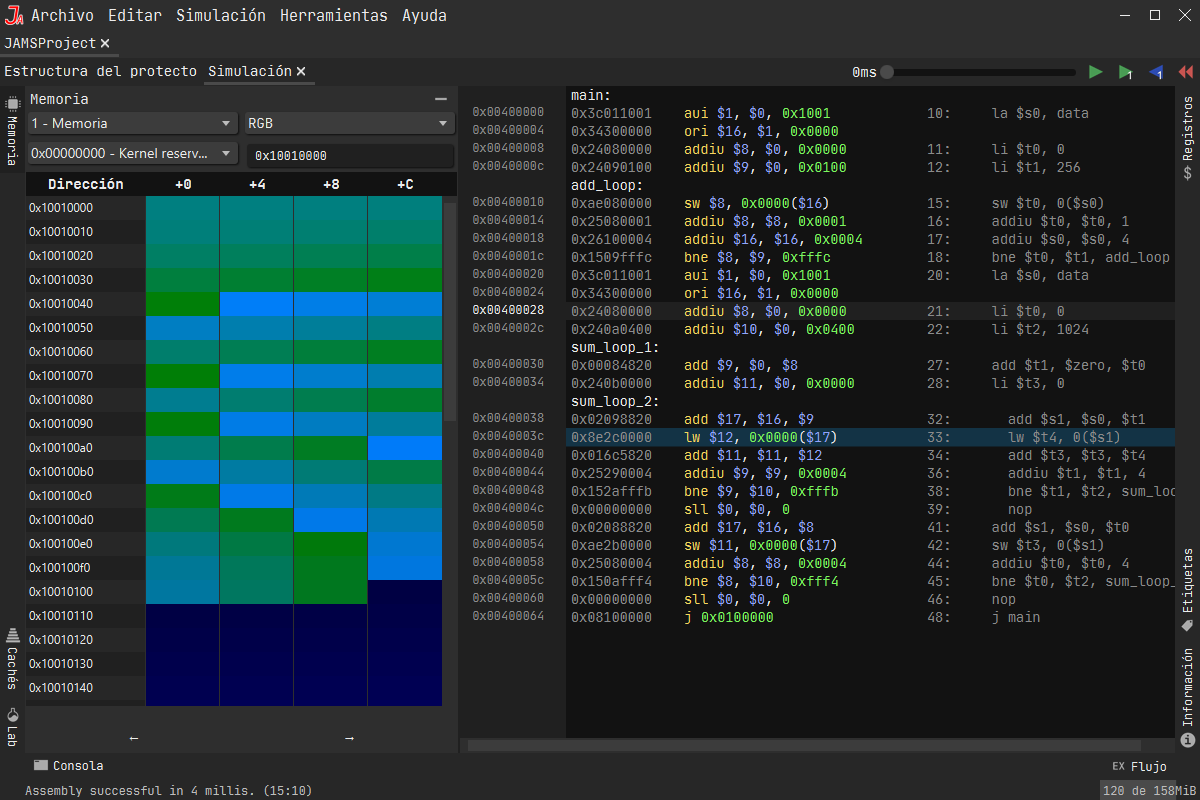
\includegraphics[width=0.8\textwidth]{images/tools/jams-memory}
    \caption{Herramienta de memoria}
    \label{fig:jams-memory}
\end{figure}

\noindent El primer desplegable de la herramienta permite elegir qué
memoria se desea visualizar.
La lista de memorias está ordenada por nivel, siendo la primera
memoria la caché de nivel 1.
Si la simulación no contiene ninguna caché,
este desplegable solo mostrará la memoria principal.

\noindent El segundo desplegable contiene diferentes opciones
en las que los datos de la memoria se puede visualizar.
Las opciones disponibles son las siguientes:

\begin{itemize}
    \item \textbf{Binario:} muestra cada valor en binario.
    \item \textbf{Caracteres:} muestra cada valor como un conjunto de
    cuatro caracteres ASCII\@.
    \item \textbf{Decimal:} muestra cada valor en decimal.
    Esta es la opción por defecto.
    \item \textbf{Coma flotante de precisión doble:}  muestra cada valor
    en coma flotante de doble precisión.
    La parte más representativa es el valor de la siguiente celda de memoria.
    \item \textbf{Texto inglés:} muestra cada valor como un texto en inglés.
    \item \textbf{Coma flotante de precisión simple:} muestra cada
    valor en coma flotante.
    \item \textbf{Hexadecimal:} muestra cada valor en hexadecimal.
    \item \textbf{Entero de 64 bits:} muestra cada valor como un número de 64 bits.
    La parte más representativa es el valor de la siguiente celda de memoria.
    \item \textbf{Octal:} muestra cada valor en octal.
    \item \textbf{RGB:} muestra cada valor como un color RGB\@.
    El cuarto más representativo del valor queda en desuso.
    \item \textbf{RGBA:} muestra cada valor como un color RGBA\@.
    \item \textbf{Romano:} muestra cada valor como un número romano.
\end{itemize}

\noindent El usuario puede desplazarse a través de la herramienta
de diferentes maneras: \textbf{seleccionando una sección}
en el tercer desplegable, \textbf{insertando una dirección}
o \textbf{usando las flechas de movimiento}.
Una vez identificado la celda deseada, el usuario podrá
\textbf{modificar su valor} haciendo doble clic en ella.
El nuevo value puede estar representado en binario, octal,
decimal o hexadecimal.


\section{Herramienta de cachés}\label{sec:herramienta-de-caches}

La herramienta \textbf{cachés} muestra información
sobre las cachés del simulador.
La herramienta está conformada por dos secciones:
las estadísticas y el registro.
En las estadísticas se muestran las operaciones,
aciertos y fallos de una caché, mientras que en el
registro se muestran todas las acciones que una
caché ha realizado junto con su resultado.

\begin{figure}[H]
    \centering
    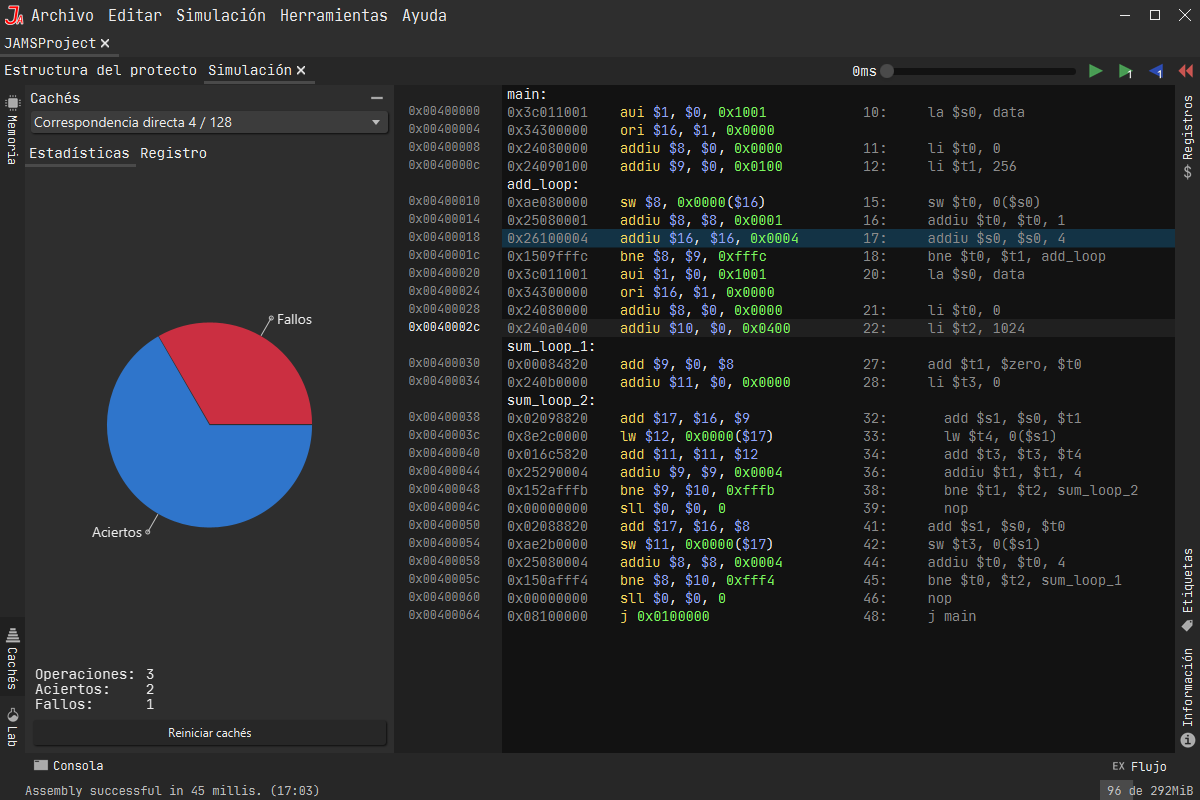
\includegraphics[width=0.8\textwidth]{images/tools/jams-caches}
    \caption{Herramienta de cachés}
    \label{fig:jams-caches-stats}
\end{figure}

\noindent A diferencia de otras herramientas, el registro no se
borra cuando se reinicia la simulación o se deshace un paso.
La herramienta está diseñada así para poder visualizar fácilmente los cambios de la caché.

\begin{figure}[H]
    \centering
    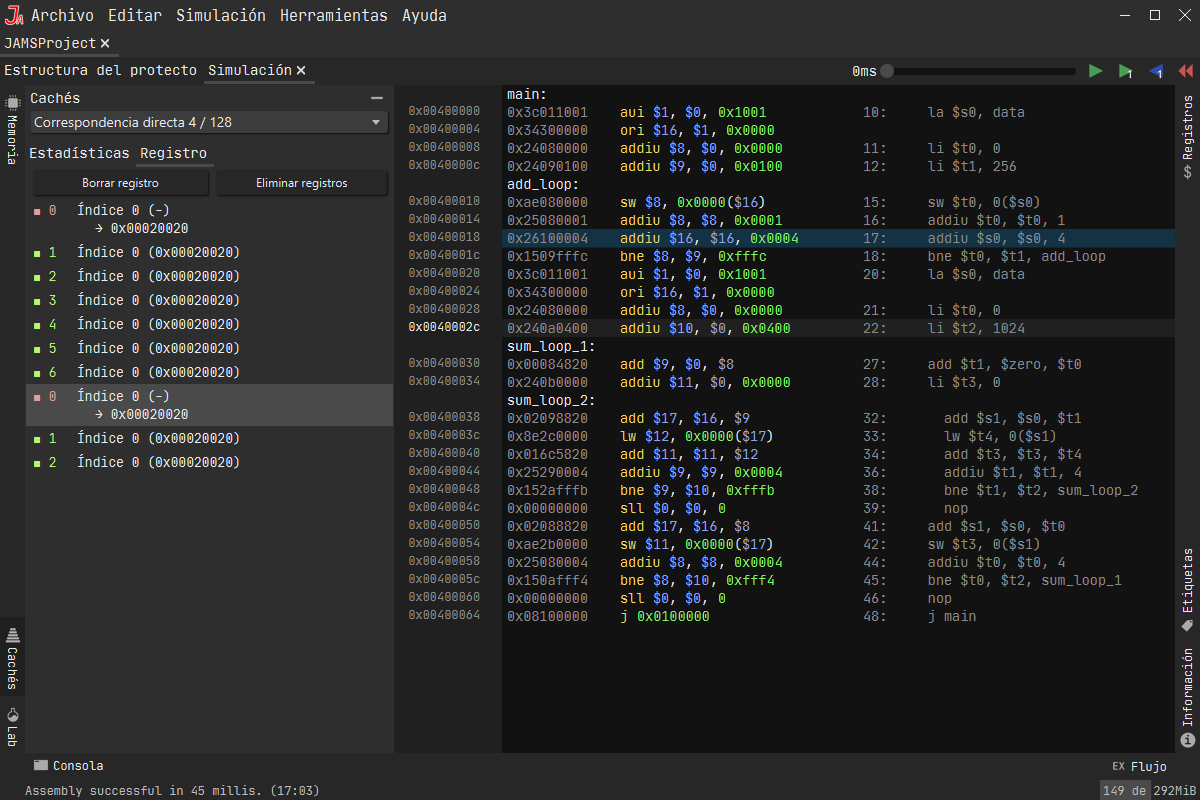
\includegraphics[width=0.8\textwidth]{images/tools/jams-caches-log}
    \caption{Registro de la herramienta de cachés}
    \label{fig:jams-caches-log}
\end{figure}

\section{Laboratorio}\label{sec:laboratorio}

La herramienta \textbf{laboratorio} simula varios componentes básicos
externos conectados a un simulador \textit{MIPS32}.
En concreto, la herramienta simula cuatro componentes básicos:
dos visualizadores de siete segmentos, un teclado hexadecimal,
un generador de interrupciones y un contador.

\begin{figure}[H]
    \centering
    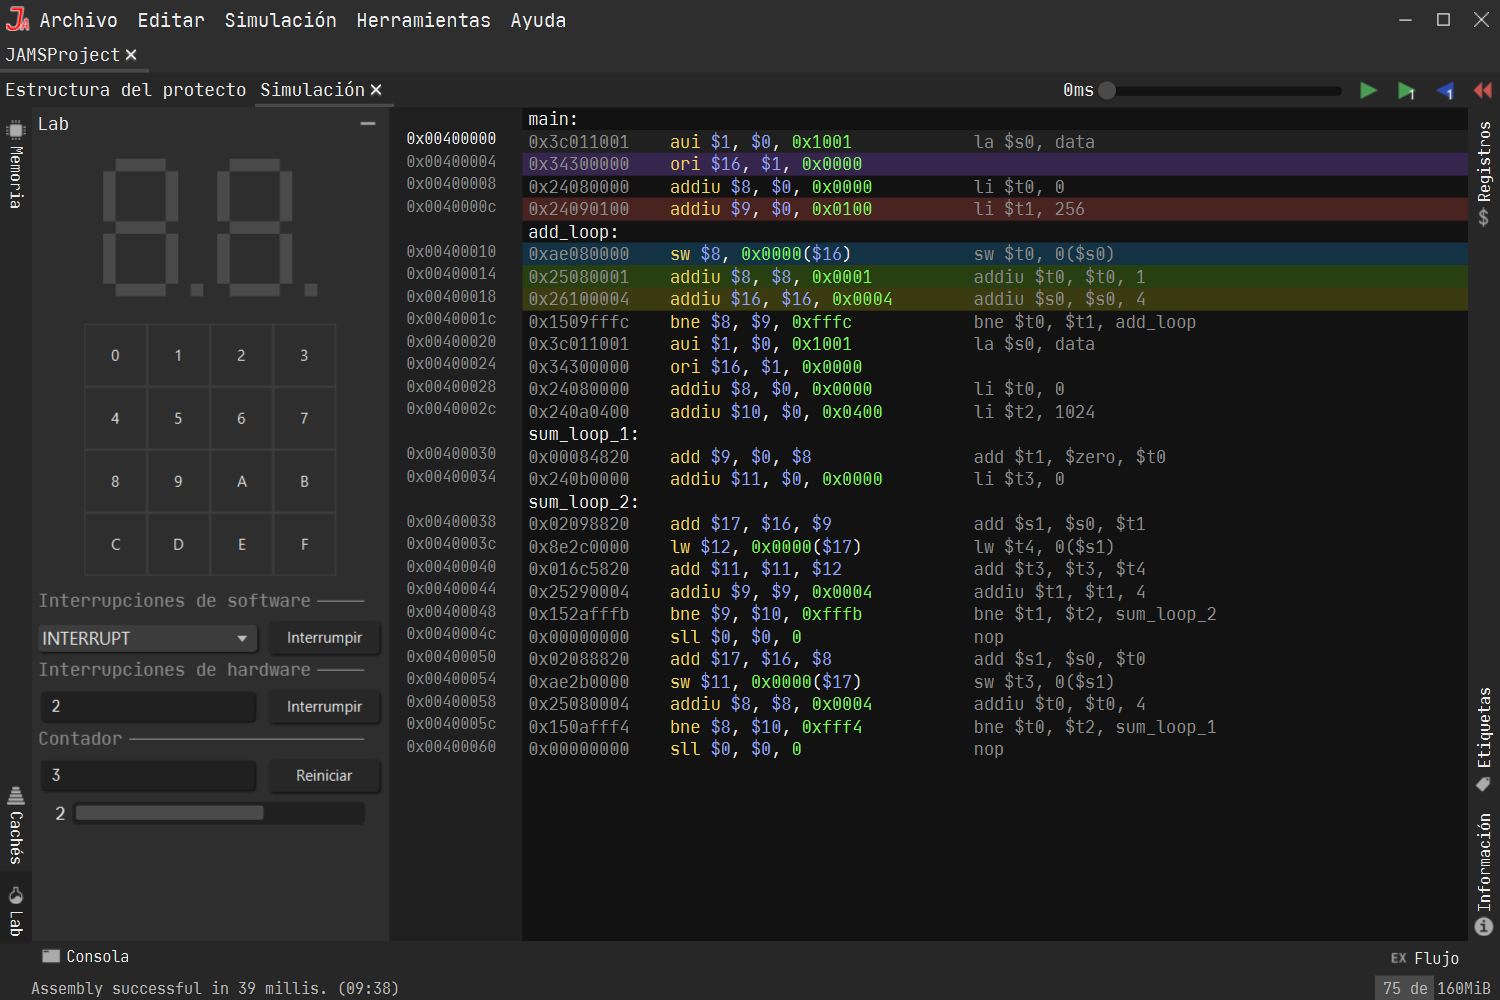
\includegraphics[width=0.8\textwidth]{images/tools/jams-lab}
    \caption{Laboratorio}
    \label{fig:jams-lab}
\end{figure}

\subsection{Visualizador de siete segmentos}\label{subsec:visualizador-de-siete-segmentos}

Un visualizador de siete segmentos \textbf{permite representar un dígito o letra},
y está controlado por el contenido de un \textbf{byte en memoria}.
En concreto, cada segmento del visualizador está controlado por un bit del byte.
Los bits que controlan cada segmento son los siguientes:

\begin{figure}[H]
    \centering
    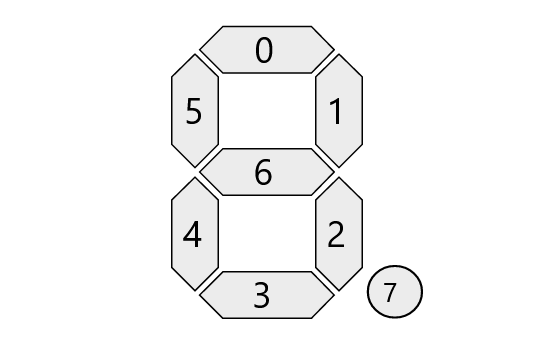
\includegraphics[width=0.5\textwidth]{images/tools/jams-seven-segment}
    \caption{Visualizador de siete segmentos}
    \label{fig:jams-seven-segment}
\end{figure}

\noindent Si, por ejemplo, se desea el dígito $5$ en el visualizador,
se debe guardar en la dirección del byte el valor $0b01101101$.

\begin{figure}[H]
    \centering
    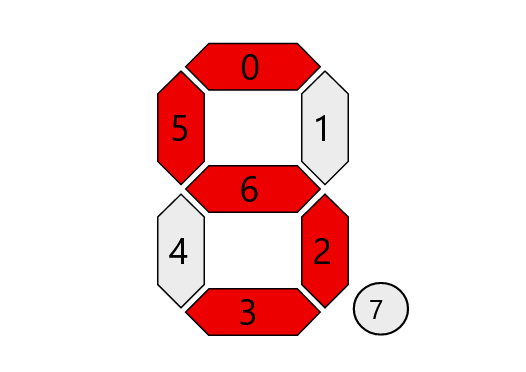
\includegraphics[width=0.5\textwidth]{images/tools/jams-seven-segment-active}
    \caption{Visualizador de siete segmentos representando un 5}
    \label{fig:jams-seven-segment-active}
\end{figure}

\noindent Las \textbf{direcciones de memoria por defecto} que controlan los dos
visualizadores son la dirección $0xffff0010$ para el visualizador derecho y
$0xffff0011$ para el visualizador izquierdo.
Estos valores se pueden cambiar en la configuración,
en el apartado \textbf{Simulación > MIPS}.

\subsection{Teclado hexadecimal}\label{subsec:teclado-hexadecimal}

El segundo componente de la herramienta es el teclado hexadecimal.
Este teclado \textbf{permite introducir valores} que el
simulador puede interpretar.
Cuando el usuario pulsa uno de los botones,
\textit{JAMS} genera una \textbf{interrupción \textit{hardware} de nivel 3}.
El programa puede interpretar el evento implementando un gestor
de excepciones en la dirección por defecto $0x80000260$.

\noindent Para saber qué \textbf{botones del teclado están activados},
se deben leer las direcciones de memoria por defecto $0xffff0013$ y $0xffff0014$.
Cada bit de los dos bytes representan un botón en el teclado.
Si un bit contiene el valor 1, el botón que representa está seleccionado.

\noindent Como ejemplo: si el valor de la dirección de memoria
$0xffff0013$ es $0b00000100$ y el valor de la dirección de memoria
$0xffff0014$ es $0b10000100$, los botones 2, A y F están seleccionados.

\subsection{Generador de interrupciones y contador}\label{subsec:generador-de-interrupciones-contador}

El generador de interrupciones \textbf{permite generar} tanto
interrupciones \textit{software} como interrupciones \textit{hardware}.
En el caso de las interrupciones \textit{software},
la herramienta permite definir la causa de la interrupción.

\noindent El contador es una pequeña herramienta
\textbf{que genera una interrupción \textit{hardware}}
de nivel 2 cada cierto número de ciclos especificados por el usuario.
Este valor se puede asignar desde la interfaz o escribiéndolo
en la dirección de memoria $0xffff0012$.

\section{Consola}\label{sec:consola}

La \textbf{consola permite ver los mensajes} de la aplicación
e introducir valores que el simulador puede interpretar.
La consola \textbf{actúa de intermediador principal}
entre el usuario y la aplicación.

\begin{figure}[H]
    \centering
    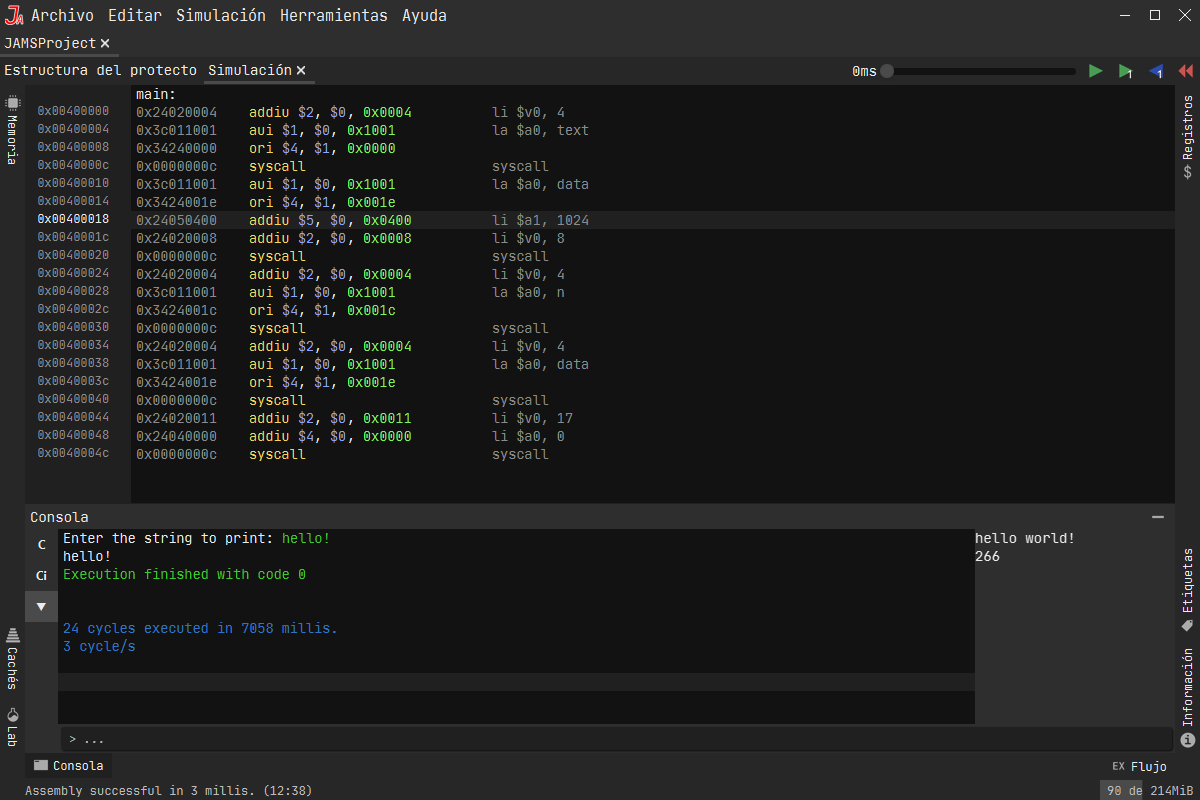
\includegraphics[width=0.8\textwidth]{images/tools/jams-console}
    \caption{Consola}
    \label{fig:jams-console}
\end{figure}

\noindent El visualizador muestra los mensajes que la aplicación
imprime mediante llamadas del sistema.
También muestra el resultado de la ejecución al terminar la simulación.
La consola permite enviar mensajes a la aplicación mediante la barra de
texto de la parte inferior de la herramienta.
Los mensajes \textbf{quedarán guardados} en una cola de mensajes
hasta que la simulación los lea.
El usuario \textbf{puede eliminar mensajes} de la cola
pulsando el mensaje que quiere eliminar.

\noindent La consola contiene tres botones con el que se puede interactuar:
\begin{itemize}
    \item El botón $C$ permite limpar el informe, eliminando todo el
    texto presente en él.
    \item El botón $Ci$ permite limpiar la cola de mensajes.
    \item El botón $\nabla$ permite habilitar o deshabilitar el desplazamiento
    automático al final del visualizador.
    Si esta opción está habilitada, el visualizador se desplazará
    automáticamente hasta el final del visualizador cuando un
    nuevo mensaje entra en él.
\end{itemize}

\section{Herramienta de flujo}\label{sec:herramienta-de-flujo}

La herramienta \textbf{flujo} permite ver el flujo de ejecución del simulador.
La herramienta tiene una funcionalidad puramente visual:
\textbf{no permite editar} ningún aspecto del simulador.
El usuario puede usar la barra deslizadora para cambiar el tamaño de las columnas,
y puede desplazarse de manera sencilla arrastrando el ratón.

\begin{figure}[H]
    \centering
    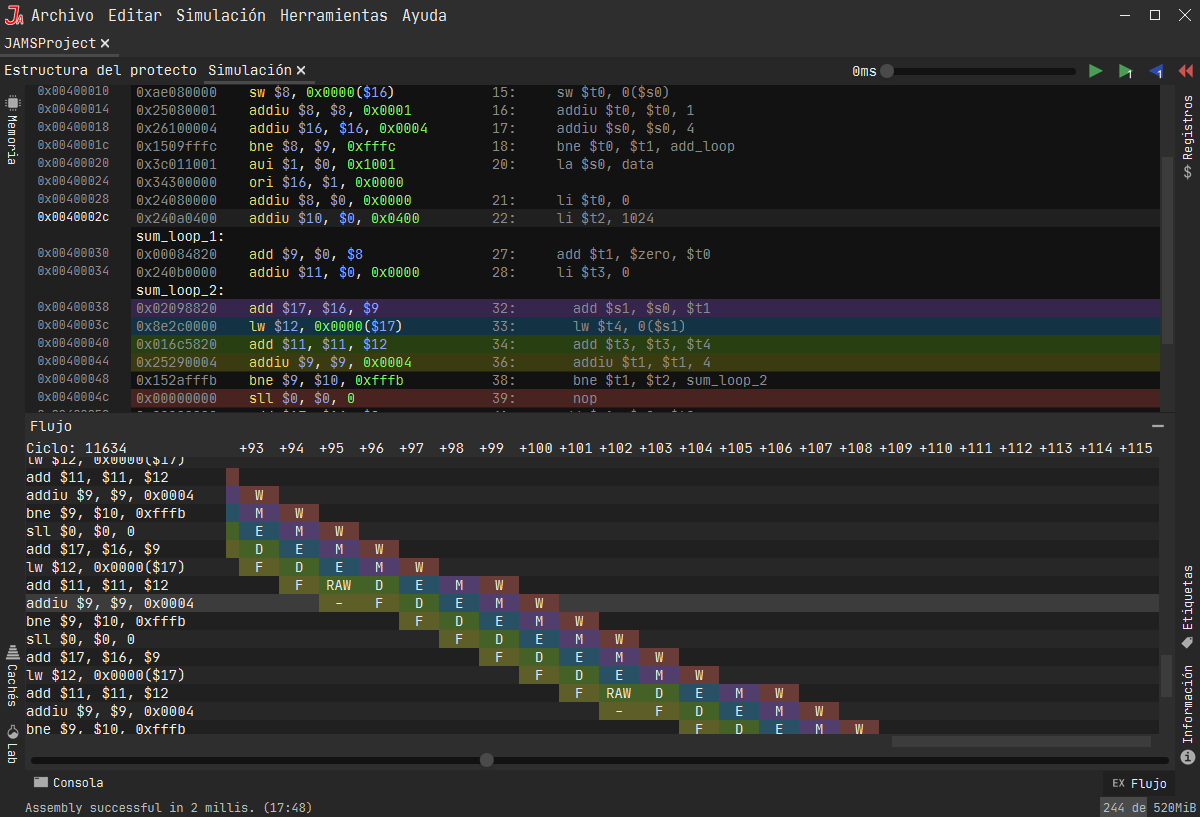
\includegraphics[width=0.8\textwidth]{images/tools/jams-flow}
    \caption{Herramienta de flujo}
    \label{fig:jams-flow}
\end{figure}

\noindent El visualizador únicamente representa un número máximo de instrucciones.
Este número es por defecto $100$, y se puede cambiar en la configuración.
El número de ciclo representado en la parte superior izquierda representa
al \textbf{primer ciclo representado por el visualizador} de flujo.
Cada columna contiene un número que representa su ciclo con respecto al ciclo inicial.

\section{Información}\label{sec:informacion}

La herramienta \textbf{información} es una herramienta muy sencilla
que informa sobre aspectos generales del simulador.

\begin{figure}[H]
    \centering
    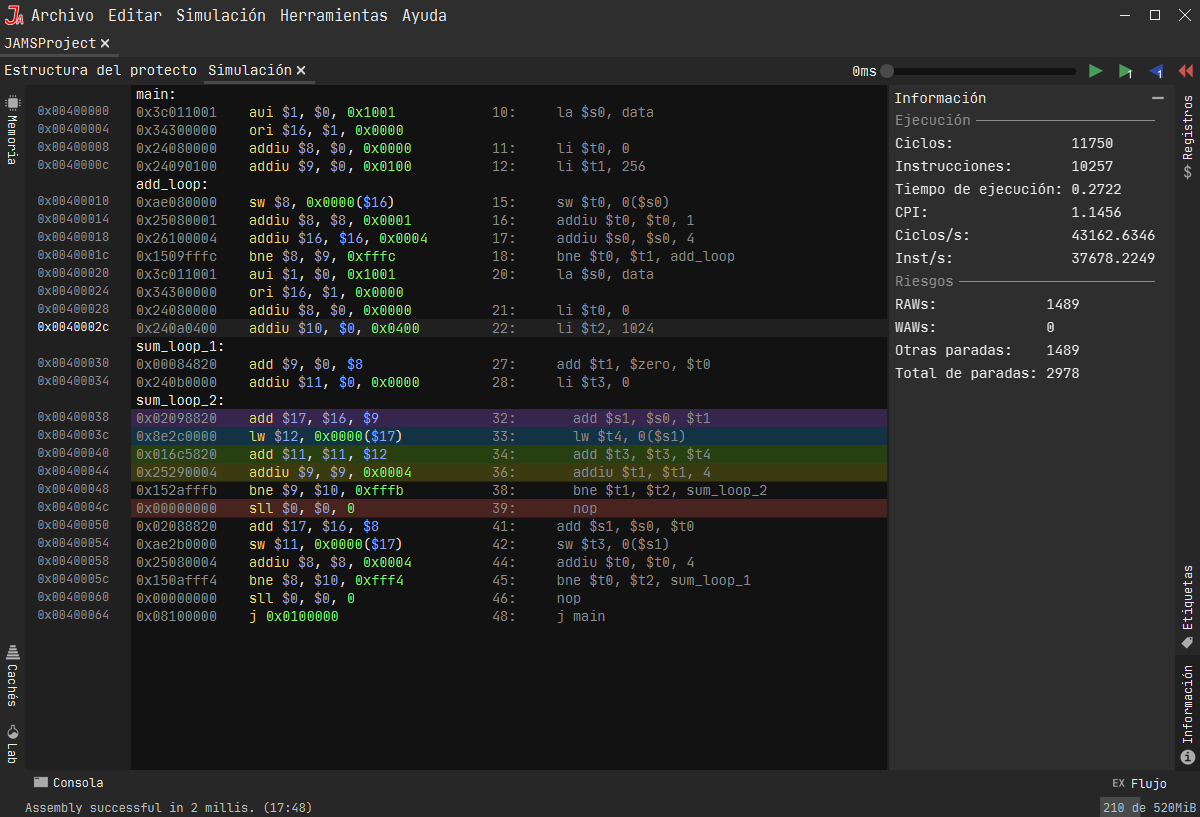
\includegraphics[width=0.8\textwidth]{images/tools/jams-information}
    \caption{Información}
    \label{fig:jams-information}
\end{figure}

\noindent La herramienta muestra los ciclos ejecutados,
instrucciones ejecutadas, tiempo de ejecución, ciclos por instrucción,
ciclos por segundo e instrucciones por segundo de una simulación.
Dependiendo del tipo de arquitectura, la simulación también podrá
\textbf{mostrar otros tipos de datos}, como los riesgos de ejecución.

\section{Herramienta de etiquetas}\label{sec:herramienta-de-etiquetas}

La herramienta \textbf{etiquetas} muestra información sobre las etiquetas
utilizadas por en ensamblador para generar la simulación.

\begin{figure}[H]
    \centering
    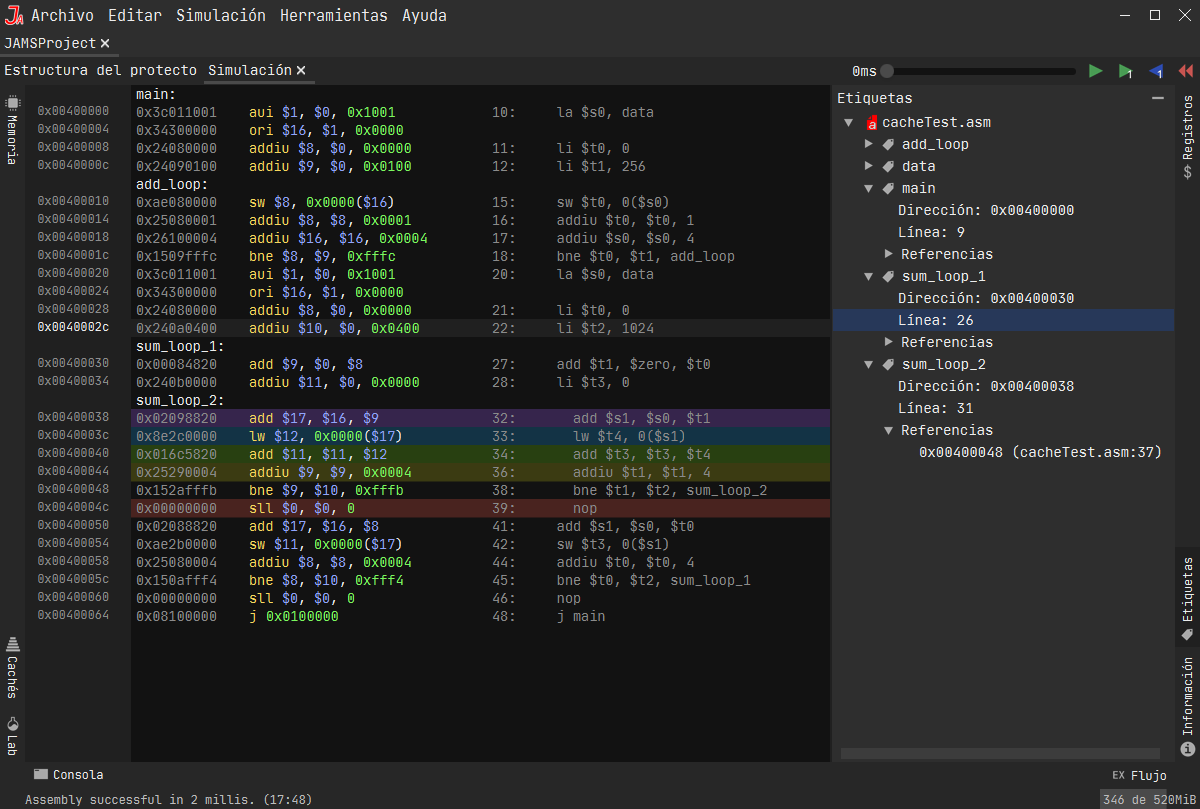
\includegraphics[width=0.8\textwidth]{images/tools/jams-labels}
    \caption{Herramienta de etiquetas}
    \label{fig:jams-labels}
\end{figure}

\noindent Las etiquetas están \textbf{catalogadas por archivos}.
Cada etiqueta contiene su dirección asignada,
la línea en la que fue declarada en el archivo y las referencias.

Cada referencia contiene la dirección en la que fue referenciada,
la línea del archivo y el archivo en sí donde se encuentra dicha referencia.
Pulsando el botón secundario del ratón sobre una etiqueta
o una referencia el usuario puede acceder al \textbf{menú de contexto}
donde se puede visualizar la dirección de memoria en el visualizador
de instrucciones o en la memoria.

\section{Herramienta de registros}\label{sec:herramienta-de-registros}

La herramienta de \textbf{registros} muestra información sobre
los registros de la simulación.

\noindent La herramienta consiste en una tabla de registros
que muestra \textbf{4 valores}: el identificador del registro,
su nombre canónico y su valor actual en decimal y hexadecimal.
En el caso de los registros del coprocesador 0,
también se muestra el sub-identificador $sel$.
En el caso de los registros del coprocesador 1,
el valor se muestra en coma flotante y no en decimal.

\begin{figure}[H]
    \centering
    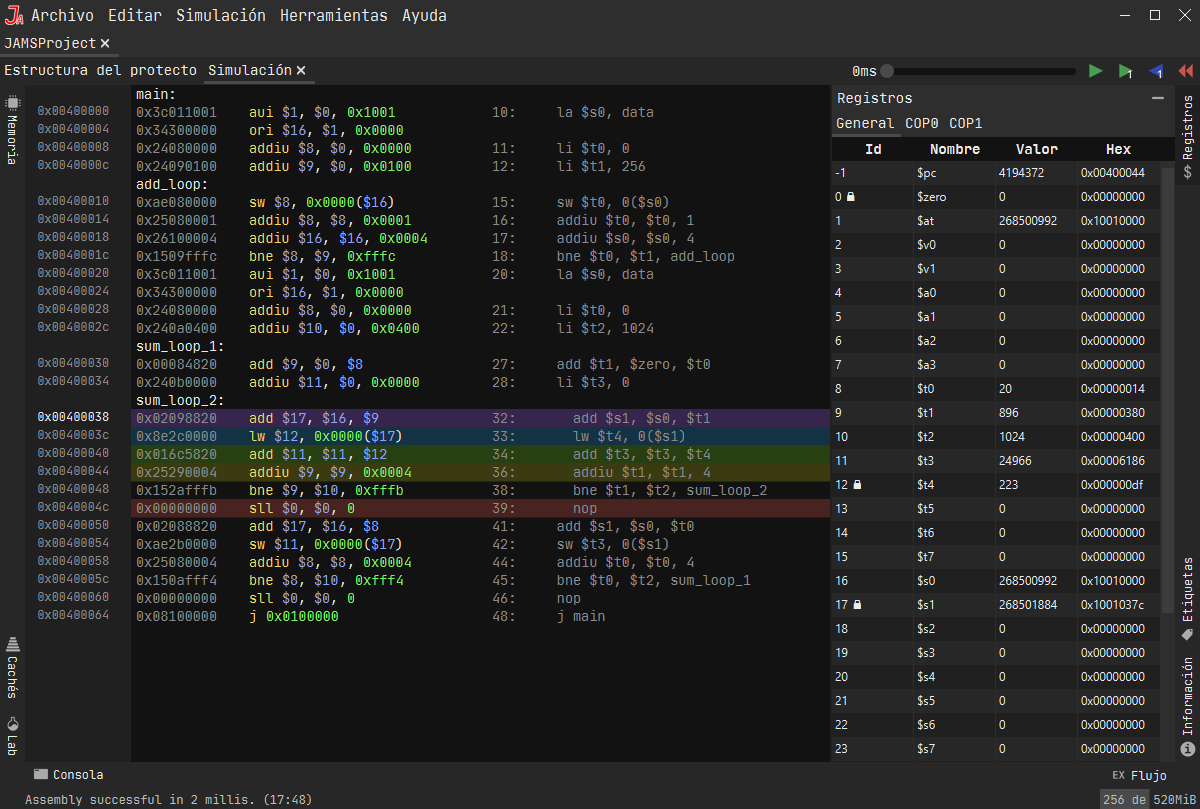
\includegraphics[width=0.8\textwidth]{images/tools/jams-registers}
    \caption{Herramienta de registros}
    \label{fig:jams-registers}
\end{figure}

\noindent En arquitecturas avanzadas, los registros pueden ser
bloqueados por una instrucción.
Cuando un registro está bloqueado, el icono de un candado \faLock \
aparecerá junto con el identificador.

\noindent El usuario puede \textbf{editar los valores de un registro}
haciendo doble clic en la casilla de valor
o valor hexadecimal correspondiente.
Al editar, el usuario puede insertar un valor en decimal,
hexadecimal, octal o binario.
En el caso de los registros del coprocesador 1,
también se pueden insertar valores en coma flotante.